\newcommand{\comment}[1]{}

%\documentclass[a4paper,twocolumn,12pt]{article}

%\documentclass[a4wide,12pt]{report}

%\documentclass[a4wide,12pt]{article}
%\documentclass[informasjonssikkerhet]{gucmasterproject}
%\documentclass[informationsecurity]{gucmasterproject}
\documentclass[informationsecurity]{gucmasterproject}

%\usepackage{pslatex} %% Doesn't seem to work - i.e. convert .eps to .pdf
 
\usepackage[utf8]{inputenc}     % For utf8 encoded .tex files
%\usepackage[latin1]{inputenc}
\usepackage[british]{babel}     % For chapter headings etc.
%\usepackage[pdftex]{graphicx}           % For inclusion of graphics

%From http://math.uib.no/it/tips/
   %% For grafikk
    \usepackage{ifpdf}
    \ifpdf
      \usepackage[pdftex]{graphicx}
      \usepackage{epstopdf}
    \else
      \usepackage[dvips]{graphicx}
    \fi
    %% Her kan du putte dine vanlige pakker og definisjoner



%\usepackage[dvips]{hyperref}    % For cross references in pdf
\usepackage{hyperref}
\usepackage{mdwlist}
\usepackage{url}
\usepackage{here}
\usepackage{subcaption}
\usepackage{cleveref}
\usepackage{makecell}

\def\UrlFont{\tt}

\begin{document}

\thesistitle{A survey of periodic authentication systems based on keyboard dynamics}
\thesisauthor{Per-Kristian Nilsen}
\thesisdate{\gucmasterthesisdate}
\useyear{2017}
\makefrontpages % make the frontpages
%\thesistitlepage % make the ordinary titlepage


\comment{
Front page - including
"   NTNU technical report front page including logos etc.
"   The text: "Specialization Report"
"   Title of project
"   Name of author and contact details
"   Date
"   Version

email address
"   MIS students must include "NISlab" as their affiliation.
Date:22.10.2003

Structure of Specialization Report
NTNU in Gj\o{}ovik
}



\begin{abstract}

User authentication based on keystroke dynamics is an active research area and several different methods have been proposed to improve the performance and viability of this authentication method.
A specific sub-category of authentication systems based on keystroke dynamics record the user's keystrokes passively during the user session and attempt to remove access if the recorded behavior does not match that of the user account's true owner.
Most of these systems analyze the typing behavior \textit{periodically}, while a few others do so continuously after every keystroke.
The possibilities of incorporating mechanisms from \textit{periodic} authentication systems into an existing \textit{continuous} authentication system are explored in this paper.
This is done by a state of the art survey, as well as detailed discussions on a selected number of proposed systems.

\end{abstract}

\tableofcontents
\chapter{Introduction}
\label{chap:introduction}

Periodic authentication (PA) based on keystroke dynamics is a growing research area with increasingly promising results.
There is a variety of mechanisms and algorithms built into published PA systems, some more successfully than others.
I will in this survey attempt to cover the state of the art and review some of the best performing PA systems, comparing them against each other.

The purpose of the survey is to prepare for my upcoming master thesis on combining continuous and periodic authentication systems.
I will there be extending the continuous authentication (CA) system proposed in Soumik Mondal's PhD thesis \cite{mondal} with a PA system in order to determine if the combination of such systems can have positive effects on performance.
Therefore, I will select PA systems to review in detail which consist of interesting and valuable functionality, or are worth discussing for other reasons.
The PA systems will be described in their entirety, though in the master thesis I will most likely be picking parts from several PA systems to be combined with the CA system.
Functionality found to be especially useful in that regard will be highlighted or discussed in each individual review.

Background information on authentication based on keystroke dynamics will be given in \cref{chap:background}, including an introductory explanation of biometrics and relevant terms used in the research field.
In \cref{chap:state}, an overview of the general state of the art will be covered.
\Cref{chap:gnp} contains a review of PA system using a statistical approach of which several other researchers have based their own systems upon.
\Cref{chap:messerman} and \cref{chap:ferreira} describe two such systems, each with their own methods for improving the original system.
A PA system based on machine learning is discussed in \cref{chap:ahmed}, before conclusions are made in an overall discussion in \cref{chap:conclusion}.


\chapter{Background}
\label{chap:background}

%NOTE PUT ANGA FORUMALS IN HERE
Biometrics is increasingly utilized for user authentication, with fingerprint readers being built into personal devices such as smart phones and laptops.
Biometric systems based on modalities such as fingerprint, hand print, iris, retina and facial recognition are to varying degrees now known to the general public.
A common feature of these modalities are that they are \textit{biological} -- they are based on our individual anatomy.
On the other hand, \textit{behavioral} biometric systems are not yet as widely used as its physiological counterpart, largely due to lesser reliability and being more prone to changes over time.

Behavioral biometrics are, as the name implies, based on the behavior of an individual. Behavioral modalities include (but are not limited to) gait recognition, voice recognition, mouse dynamics and keyboard dynamics, with the latter being the focus of this literature study.
'Keyboard dynamics' is a term revolving around capturing the features from a person's typing rhythm, and using them for purposes such as user authentication, identification and classification.
\textit{Identification} means determining whether or not a person is a known user of a system, and if so, who it is.
\textit{Classification} is the process of determining who a person is within a set of possible individuals, while \textit{authentication} is verifying whether or not a person is who they claim to be.

These systems may be used either to \textit{give access} or to \textit{remove access}.
Similar to password based authentication, keystroke dynamics can be utilized for initial \textit{static (one-time) authentication}, \textit{giving} a legal user access to their system if it is apparent that the typing user is the \textit{genuine} user of the claimed identity.
One approach to this kind of authentication is having a user write a predetermined and fixed sample text of which typing features are extracted to form a probe to be compared to their previously enrolled reference.
The text may be short or long, depending on the authentication system at hand.  
An example of a short text may the user's password, while long text could be a short news article.

\textit{Dynamic authentication} generally takes place after static authentication, and \textit{removes access} if the current user is believed to be an imposter, i.e. someone other than the genuine user of the logged in account.
The user is repeatedly authenticated throughout their session, as an additional layer of security on top of the static authentication.
Again, both fixed- and free-text can be used for this purpose.
There are two approaches to free-text dynamic authentication, namely \textit{continuous} and \textit{periodic} authentication, both of which rely on passively monitoring the user's typing behavior, and determining whether the current user is the genuine user of the logged-in account.
Periodic authentication (PA) systems rely on passively recording a \textit{block} sample of keystrokes of which features are extracted from to generate a probe when the block is filled.
These features are then compared to the reference, similarly to the static authentication systems previously mentioned.
The authors of PA systems have a tendency of calling their methods "continuous authentication" (CA), but as Bours \cite{BOURS201236} pointed out, the term "continuous" implies that the authentication process is performed after each individual keystroke.
I will therefore refer to all PA systems in the literature as "periodic", regardless if the authors themselves refer to their methods as "continuous".

CA systems such as the one proposed in \cite{BOURS201236} only considers the last keystroke plus its relation to the keystroke before (if any).
Similarly to PA systems, these features are then compared to the reference. 
However, CA systems have much less statistics to work with compared to PA systems.
The upside to CA systems is that they react instantly to every user action, such as increasing or lowering the trust in the user's genuineness in Bours' system \cite{BOURS201236}.
On the contrary, PA systems cannot react to impostors until enough keystrokes have occurred to fill the block.
Until that happens, the impostor has free reign over the genuine user's account in the system.

The features extracted from keystrokes vary between different systems.
For single key actions, there are two events happening, namely Key Down and Key Up, which means pressing and releasing the key, respectively.
Timestamps are associated with these events, usually at the granularity of milliseconds.
From these timestamps, the \textit{dwell time} of the keypress can easily be determined.
When two or more sequential keypresses (n-graphs) are to be considered in relation to each other, a number of features can be extracted.
As an example, the \textit{digraph} 'AB' may have the timing values as shown in \cref{tab:timing-example}.
From those values, one could extract the dwell times of the single keys, but also the following features called \textit{digraph latencies}: 

\begin{itemize}
\item $lat\textsubscript{dd} = B\textsubscript{down}-A\textsubscript{down} = 125ms-80ms = 45ms$
\item $lat\textsubscript{du} = B\textsubscript{up}-A\textsubscript{down} = 140ms-80ms = 60ms$
\item $lat\textsubscript{ud} = B\textsubscript{down}-A\textsubscript{up} = 125ms-100ms=25ms$ (also called flight time)
\item $lat\textsubscript{uu} = B\textsubscript{up}-A\textsubscript{up} = 140ms-100ms=40ms$
\end{itemize}
where for example lat\textsubscript{du} refers to the \textit{down-up} latency.
In other words, this is the latency between pressing down the first key (A), and releasing the second key (B).
The authentication system could then use these features to calculate the similarity to the reference template for instance by using one or more distance measures, or by using machine learning algorithms.

\begin{table}[h]
    \centering
    \begin{tabular}{lll}
         \bf Key & \bf Action & \bf Timestamp (ms)\\
         A & Down & 80\\
         A & Up & 100\\
         B & Down & 125\\
         B & Up & 140
    \end{tabular}
    \caption{Example timing values for 'AB' digraph.}
    \label{tab:timing-example}
\end{table}

Another difference between PA and CA systems in literature is the way performance is reported.
False Accept Rate (FAR), False Reject Rate (FRR) and Equal Error Rate(EER) are generally used for indicating the performance of PA classification algorithms.
FAR represents the percentage of imposters being falsely accepted, which indicates the security level of the system. 
FRR represents the percentage of genuine users being falsely rejected, which has implications for user acceptance, as being rejected too often would be a source of irritation.
These two rates are inversely proportional to each other, as lowering the FAR inherently increases the FRR.
The ERR therefore shows the point where the FAR and FRR of a system have the same value.
These rates must be looked at in relation to the PA system's block size in order to be meaningful.
I would also like to mention that much of the PA literature misuses the FAR and FRR terms, as they are system-level evaluation metrics, and they are often wrongly used to describe the performance of their classification algorithms.
According to the vocabulary specified in the ISO/IEC 2382-37 standard \cite{ISO-voc}, the correct terms for algorithm level performance is False Match Rate (FMR) and False Non-Match Rate (FNMR), and I will replace wrongly used terms where applicable when discussing the literature.

Bours and Mondal proposed in 2015 two new metrics for evaluating the performance of CA systems, namely Average Number of Imposter Actions (ANIA) and Average Number of Genuine Actions (ANGA) \cite{CA-performance}.
These rates look at how many actions imposters and genuine users on average can perform before being rejected by the authentication system, as it often is more useful to know how often users will be locked out than the probability of that happening per sample.
They also provide the following formulas for converting PA systems' FAR into ANIA rates and FRR into ANGA rates.

\begin{equation}
ANIA = \frac{block size}{(1-FMR)}
\end{equation}

\begin{equation}
ANGA = \frac{block size}{FNMR}
\end{equation}

The performance metrics used in Mondal's \cite{mondal} CA system is ANIA and ANGA, and I will therefore use the conversion formulas from \cite{CA-performance} in order to easily compare the performance of PA systems to the CA system's performance.

%NOTE: MOVE ANIA / ANGA to Background


%\chapter{Project description evaluation criteria}

%\chapter{Enrollment}
%The enrollment phase of the different papers written on periodic authentication have varying approaches to collecting data for generating reference templates.
%This chapter will cover the approaches most relevant to my master thesis and contain a discussion on which of them, if any, are applicable.
%
%After gathering participants, their keystroke data must be recorded.
%In my case, this phase will last a longer period of time, as the data will be recorded in a completely uncontrolled environment.
%Specifically, the participants will be installing software on their private computers, and the software will record all keyboard activity for as long as the enrollment phase lasts.

%\chapter{Feature extraction}
%While the CA system will consider timing data for monographs, the PA system will likely have focus on digraphs, or possibly n-graphs of greater length.


\chapter{State of the art}
\label{chap:state}
This section gives an overview of the state of the art, and the different methods and approaches taken by researchers.
While this literature study has a focus on PA systems, I have also included CA \cite{BOURS201236, mondal} and periodic identification systems \cite{Solami, Janakiraman2007, Monrose} in the state of the art, as they are relevant to the topic.
Periodic authentication and periodic identification are different in terms of the classification algorithms used, as identification systems need to compare the typing behavior of the current user to every legal user in the system in order to determine who it is.
Even if the classification algorithm is inappropriate for authentication systems, these systems are relevant as they may use comparison methods such as distance measures and machine learning, which can also be used for PA.

\section{Data collection}
A large portion of the PA (and CA) authentication systems in literature had participants writing text freely during the data collection phase of the experiments, with the exception of one \cite{hu} using static text.
Writing static text refers to typing a pre-determined text, which is generally done by having all participants manually typing the same long text as they are reading it.

Of the free-text studies, several were performed in an unconstrained manner \cite{superResults, Pinto2014, Ahmed, Janakiraman2007, BOURS201236, mondal, sliding}, meaning that the collection was performed in the background of participants' own computers as they were performing their usual tasks.
One study captured keystrokes in the background of an e-mail application \cite{Messerman}.
Some studies used keystroke data collected from a webform where participants were asked to write text freely before submitting the content to the researchers \cite{gnp, davoudi2009, davoudi2010, Solami}.
Certain studies were found where the researchers gave the participants pre-defined tasks to perform while the keystroke data was being collected \cite{900words, Monrose, monaco, park, KIM2017}, for example writing fictional e-mails.
One of these studies \cite{KIM2017} simulated free-text typing by assigning \textit{different} long texts to all participants, which they then were to write themselves while reading.

While most studies have not openly shared their collected keystroke data, there exists at least three open databases containing free-text keystroke data: 
\begin{itemize}
    \item Vural et al.'s \cite{vural} database contains around 840 000 keystrokes collected from 39 users over the course of two months.
    
    \item Gunetti and Picardi's \cite{gnp} complete database contains around 480 000 keystrokes from 40 users collected over a time span of six months. However, only 21 of those users agreed to have their keystroke data published \cite{Solami}.
    
    \item Huang et al.'s \cite{sliding} database contains around 9.7 million keystrokes from 95 users over the course of two years.
\end{itemize}
Researchers have generally performed their own data collection, though at least three studies \cite{davoudi2009, davoudi2010, Solami} used Gunetti and Picardi's \cite{gnp} dataset, excluding their own study.
Eleven studies involved 30 participants or more \cite{gnp, Messerman, superResults, Ahmed, 900words, KIM2017, Monrose, sliding, mondal, monaco, park}, one of which involved 2000 users \cite{900words}.

\section{Feature extraction}
All of the mentioned studies extracted feature vectors using various types of latencies between consecutive keystrokes, however nine of them \cite{superResults, Pinto2014, Ahmed, KIM2017, Janakiraman2007, Monrose, BOURS201236, mondal, monaco} also extracted dwell times of single key actions.
For consecutive keystrokes, eleven studies \cite{davoudi2009, davoudi2010, Ahmed, KIM2017, Solami, Janakiraman2007, Monrose, BOURS201236, mondal, monaco, park} considered only digraphs, one considered only trigraphs \cite{900words}, while the rest considered n-graphs with multiple values of n where $1<n$.

Out of the periodic authentication and identification systems, the block length used for feature extraction of probes was 500 keystrokes or less in seven studies \cite{Messerman, superResults, Pinto2014, Ahmed, hu, park}.
Instead of using a fixed block length, Huang et al. \cite{sliding} proposed a time-based PA system which performs an authentication every minute, examining all keystroke actions performed during the last minute of the user session.
This is a form of \textit{sliding window}, which is discussed in \cref{chap:conclusion}.

\section{Method}
Many studies have used statistical approaches to classification, while others utilize machine learning methods. 
Gunetti and Picardi's \cite{gnp} R and A measures have been utilized in several researches \cite{gnp, superResults, Pinto2014, hu, sliding}.
The R and A measures are described in \cref{chap:gnp}.
One study only adopted the R measure \cite{Messerman}, while two studies applied their own customizations to the R measure \cite{davoudi2009, davoudi2010}.
Other distance metrics used in literature are Euclidian \cite{Monrose}, Scaled Euclidian \cite{mondal}, Scaled Manhattan \cite{BOURS201236}, Bhattacharyya \cite{Janakiraman2007} and Correlation \cite{mondal} distances.
Park et al. \cite{park} used a Kolmogorov-Smirnov Test as their classifier.
\textit{K-means clustering} was used for classification in \cite{KIM2017, Solami}, and \textit{kernel ridge regression} was utilized in \cite{900words}.
Two studies have used the \textit{neural network} machine learning algorithm \cite{Ahmed, mondal}, where one of those studies also used a \textit{support vector machine} \cite{mondal}.
Lastly, two studies applied the \textit{k-nearest neighbor} lazy learning algorithm \cite{hu, monaco}.
All the systems mentioned in this chapter are summarized in \Cref{tab:state}.


%NOTE: sjekk om Hu ikke har free-text
%NOTE: husk å fikse UNCONSTRAINED i hele greien.



%NOTE: \cite{Messerman} and \cite{superResults} periodically updates user profiles.
%NOTE: \cite{900words} experiments made final decision after all words in test set were considered.
%NOTE: \cite{superResults} has asynchronous authentication


%NOTE: http://onlinelibrary.wiley.com/doi/10.1002/cpe.3718/full HAS A GOOD OVERVIEW OF STATE OF THE ART. 
%NOTE: http://www.sciencedirect.com/science/article/pii/S1568494617305847 THIS ONE TOO
%NOTE: https://www.hindawi.com/journals/tswj/2013/408280/ HAS A LOT OF DIFFERENT POINTS TO TALK ABOUT IN STATE OF ART
\begin{table}[h]
\resizebox{\textwidth}{!}{%
\begin{tabular}{ |l|p{2.1cm}|l|p{2.15cm}|p{3cm}|p{2.3cm}|p{2.5cm}|l| } 
 \hline
 \bf Paper & \bf Block length & \bf Users & \bf Task & \bf Method & \bf Performance & \bf Feature & \bf DB \\ \hline
 \cite{gnp} & 700-900 & 40 & Webform & R and A measures & FMR 0.005\% FNMR 4.833\% & 2-, 3- and 4-graph latency & Own*\\ \hline
 \cite{Messerman} & 50 - 150 & 50 & Webmail & R measure & FMR 2.02\%  FNMR 1.84\% & n-graph latency & Own\\ \hline
 \cite{superResults} & 250 & 60 & Unconstrained & R and A measures & EER 1.4\% & Dwell time, flight time for 2-, 3-, and 4-graphs & Own\\ \hline
 \cite{Pinto2014} & 150 & 10 & Unconstrained & R and A measures & FMR ~2\% FNMR ~2\% & Dwell time, flight time for 2-, 3-, and 4-graphs & Own \\ \hline
 \cite{davoudi2009} & 700-900 & 21 & Webform & Modified R measure & FMR 0.08\% FNMR 18.8\% & Digraph latency & \cite{gnp} \\ \hline
 \cite{davoudi2010} & 700-900 & 21 & Webform & Weighted R measure & FMR 0.07\% FNMR 15.2\% & Digraph latency & \cite{gnp} \\ \hline
 %Singh &- & - & - & - & - & STATIC AUTHENT. DONT BOTHER & \\ \hline
 %Kaneko \cite{Kaneko} & ~200 & 51 & No & Euclidian & 0.66\% EER & Static fixed text, jap. & di \\ \hline
 \cite{Ahmed} & 500 & 53 & Unconstrained & Neural Networks (NN) & FMR 0.0152\%, FNMR 4.82\%, ERR 2.13\% & Dwell time, digraph flight time & Own\\\hline
 \cite{hu} & 36 & 19 & Webform, static text & R and A measures, k-Nearest Neighbor & FMR 0.045\% FNMR 0.005\% & n-graph latency & Own \\ \hline
 \cite{900words} & 900 words & 2000 & Pre-defined tasks & Kernel Ridge Regression, truncated-RBF kernel & EER 1.39\% & Trigraph flight times & \cite{chang} \\ \hline
 \cite{KIM2017} & 1000 & 150 & Pre-defined task & K-means clustering & EER 0.44\% & Dwell time, digraph latencies & Own \\ \hline
 %\cite{CPE3718} & 14 & 31 & Password & MLP Neural Network & EER 0.051\% & Static auth \\ \hline
 \cite{Solami} & 700-900 & 14 & Webform & K-means clustering & Accuracy 100\% & Digraph latency & \cite{gnp}\\ \hline
 \cite{Janakiraman2007} & Minimum 2 & 22 & Unconstrained & Bhattacharyya distance & Accuracy 70\%-100\% & Dwell time, digraph flight time & Own\\ \hline
 \cite{Monrose} & Unknown & 31 & Pre-defined tasks & Euclidian distance, weighted probability & Accuracy 23\% & Dwell time, digraph flight time & Own\\ \hline
 \cite{sliding} & 1 min sliding window & 56 & Unconstrained & R and A measures & FMR 1\% FNMR 11.5\% & n-graph latency & Own*\\ \hline
 \cite{BOURS201236} & Continuous & 25 & Unconstrained & Scaled Manhattan distance & 182 ANIA & Dwell time, digraph latency & Own\\ \hline
 \cite{mondal} & Continuous & 53 & Unconstrained & Scaled Euclidian distance, Correlation distance, NN, support vector machine & 499 ANIA, 16057 ANGA & Dwell time, digraph latencies & Own \\ \hline
 \cite{monaco} & 775 on average & 119 & Pre-defined tasks & k-Nearest Neighbor & EER 3.7\% & Dwell time, digraph latencies incl. flight time & Own \\ \hline
 \cite{park} & 300 & 35 & Pre-defined tasks & Kolmogorov-smirnov Test & EER 0.09\% & Digraph latency & Own \\ \hline

\end{tabular}
}
\caption{Summary of state of the art in PA and CA systems. In the database (DB) column, systems marked with a star * have released their database to the public. This table is also presented in my Research Project Planning report.}
\label{tab:state}
\end{table}

% Enrollment size:
% \cite{KIM2017} 5000 keystrokes


\chapter{Gunetti \& Picardi}
\label{chap:gnp}
An interesting method for authenticating users was proposed by Gunetti \& Picardi in 2005 in a paper which became highly cited due to its promising results \cite{gnp}.
Their system uses two distance measures, namely absolute (A) and relative (R) measures between samples.
The R and A measures are summed to produce a final distance.
Following is a summary of how the R and A measures are calculated.

Given an attempt sample and a stored sample, a probe and reference is built by extracting the n-graphs shared by both samples into feature vectors sorted by n-graph latency (for instance \textit{down-down} latency).
The relative distance between the probe and reference can then be calculated as follows.
The position of each n-graph in the probe is compared to the position of the same n-graph in the reference, producing a position distance for every n-graph.
The position distances between all the n-graphs are then summed before being normalized, resulting in an R measure.
Normalization is performed by dividing the summed differences by the maximum disorder possible in an array with length equal to the number of shared n-graphs.

\begin{figure}[h]
    \centering
    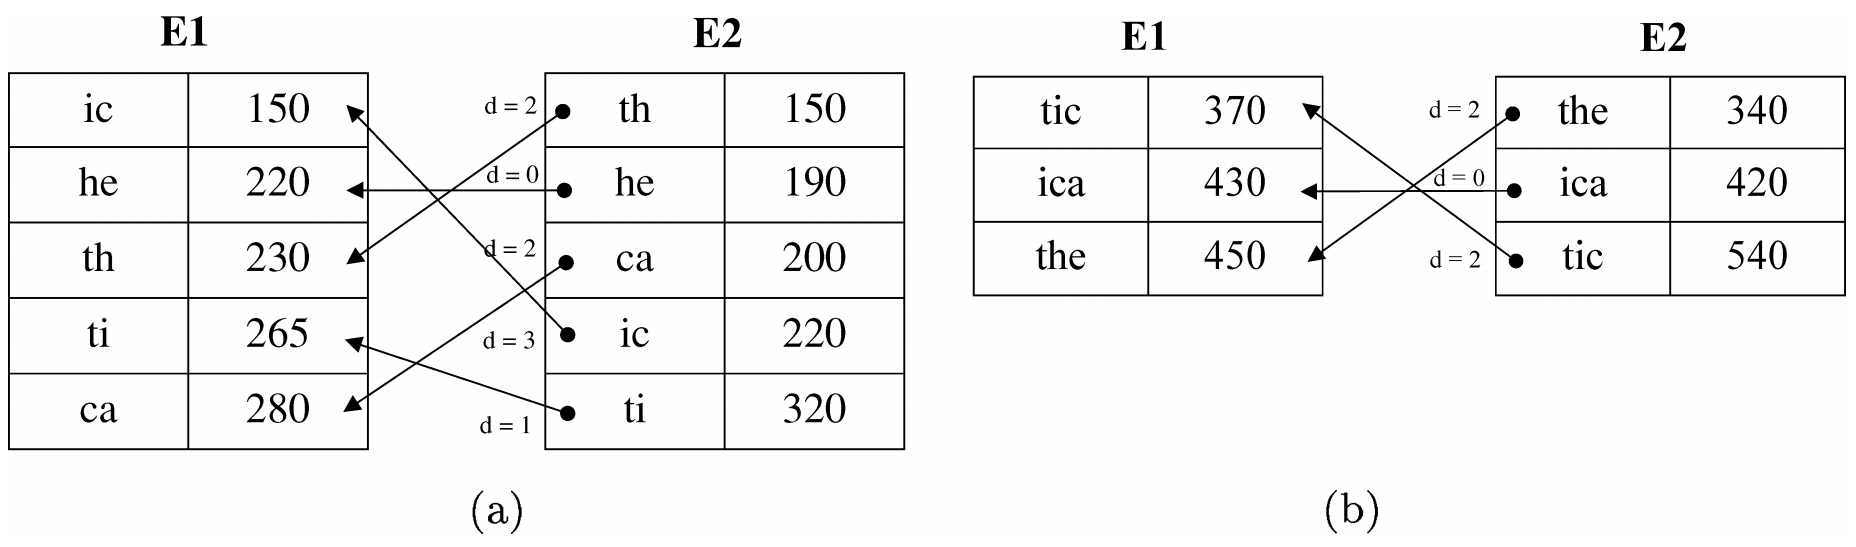
\includegraphics[width=1\textwidth]{gunetti/R-measure}
    \caption{Computation of relative distance between samples with shared digraphs (a) and trigraphs (b), as presented in \cite{gnp}.}
    \label{fig:R-measure}
\end{figure}

\Cref{fig:R-measure} demonstrates the comparison between samples.
An attempt sample containing the word \textit{authentication} and a stored sample containing the word \textit{theoretical} have their shared n-graphs extracted into the respective feature vectors E1 and E2.
Shared digraphs are shown in (a) and shared trigraphs are shown in (b). 
As pointed out by the authors, the summed position distances in (a) is $2+0+2+3+1=8$.
As there are five shared digraphs, the maximum disorder of the array is $(5^2-1)/2=12$.
Therefore, the R distance between E1 and E2 in (a) is $8/12 = 0.666$.

A method for combining relative distances based on more than one n-graph is also provided, where the relative distances of the different n-graphs are weighed based on the number of shared n-graps they contain. 
In the example above, (a) and (b) would be combined by summation with weights 5 and 3, respectively.
The reason for these weights is that a distance becomes more meaningful as the number of n-grams it is based on increases, and (a) is in this case the more meaningful case.

The authors state that the purpose of the R measure is to account for differences in typing speed that affect all n-graphs similarly.
They explain this with the example of someone with a headache possibly typing slower, but doing so for all text they input.
It is worth mentioning that this could also be the case if the subject has cold fingers, is under the influence of alcohol or other substances, or a number of other factors.
While everything is typed slower, the \textit{relative} speed between different n-grams in the same sample is likely to be similar to the relative speed between n-grams in another sample where they were typing at normal speed.

On the other hand, the A measure takes the absolute speed of corresponding n-graphs in two samples into account, as the absolute speed of an imposter's typing pattern is less likely to be similar to the reference than that of the genuine user.
For this measure to be calculated, shared n-graphs in an attempt sample and stored sample are compared and deemed to either be \textit{similar} or not.
If the latencies for these n-graphs are different from eachother, they are regarded as \textit{similar} if the longer latency divided by the shorter latency is between 1 and an arbitrary threshold.
Their reason for using a threshold instead of relying on standard deviation is that it enables them to use n-graphs which only occur once in the samples.
The authors chose 1.25 as the threshold for their experiments after testing various thresholds on the data of the five first subjects in their experiment, to avoid overfitting.
Then, they define the A measure of two samples as 1 -- (number of similar n-graphs between the samples) / (total number of n-graphs shared between the samples).

For example, for the (b) case in \cref{fig:R-measure}, we can calculate the A measure with a threshold of 1.25 as seen in \cref{tab:gnp-similar}.
The only similar trigraph pair is 'ica', which means that the A measure for E1 and E2 is $1-(1/3)=0.66$.
In a case where the threshold was set to 1.35, both the 'ica' and 'the' pairs would be regarded as similar, resulting in an A distance measure of $1-(2/3)=0.33$.
\begin{table}[h]
\centering
\begin{tabular}{ccccc}
 \bf Trigraph & \bf E1 & \bf E2 & \bf Calculation &  \\
 tic & 370 & 540 & $540/370=1.46$ &  \\
 ica & 430 & 420 & $430/420=1.02$ & (similar) \\
 the & 450 & 340 & $450/340=1.32$ & 
\end{tabular}
\caption{Similarities between trigraphs from \cref{fig:R-measure}.}
\label{tab:gnp-similar}
\end{table}

\section{Experimental setting}
For their experiment, they had 40 volunteers submitting 15 samples each, consisting of text written in a webform. On average, the sample length was around 800 characters.
14 of these samples were used to build a user profile, while the remaining sample was used as a probe.
Another 165 volunteers were asked to provide only one sample each, which was to be used as impostor samples for attacking the genuine user profiles.
The users were asked to only submit one sample per day, though they were free to wait longer between each sample.
The samples were generally collected from the volunteers' workstations and notebooks, and were all written as free-text.

\subsection{Algorithm}
\label{sec:gnp-algorithm}
Suppose a user is claiming the identity of a specific user A (by being logged into A's account) produces a sample X with a certain \textit{mean distance} to every sample in A's profile, denoted by md(A,X).
For X to be recognized as a genuine sample from user A, both of the following requirements must hold \cite{gnp}:

\begin{enumerate}
\item md(A,X) is the smallest with respect to any other md(B,X), where B is another legal user of the system.
\item md(A,X) is smaller than the mean distance between all samples in A's profile m(A), \textbf{or} md(A,X) is closer to m(A) than to any other md(B,X).
\end{enumerate}
Involving all users in the process is rather counterintuitive for an authentication algorithm.
This is further discussed in \cref{sec:gnp-scalability}.
\subsection{Performance}
The best performance of their system was achieved using a summation of R and A distances for 2-, 3-, and 4-graphs, reaching an FMR of 0.005\% and an FNMR of 4.833\%, though they call the rates "Imposter Pass Rate (IPR)" and "False Alarm Rate (FAR)".
By using the formulas mentioned in \cref{chap:background}, we can convert these rates to ANIA and ANGA rates: $ANIA = \frac{800}{(1-0.00005)} \approx 800$ and $ANGA = \frac{800}{0.04833} \approx 16553$.
The ANGA rate of 16553 is a positive result, though the ANIA rate of 800 is a clear issue.
This is further discussed in \cref{sec:gnp-blocksizes}.

%\begin{equation}
%ANIA = \frac{block size}{(1-FMR)} = \frac{800}{(1-0.00005)} \approx 800
%\end{equation}
%
%\begin{equation}
%ANGA = \frac{block size}{FNMR} = \frac{800}{0.04833} \approx 16553 
%\end{equation}

\section{Discussion}
\subsection{Scalability issues}
\label{sec:gnp-scalability}
An issue with Gunetti \& Picardi's method is that during authentication, it compares a probe to every user profile in the system.
This is of course necessary in identification situations where the system is trying to determine which user is typing, provided that no identity has been claimed in advance.
This is indeed very similar to the method they used for identification, however, comparing a sample to every user profile in the system introduces quite severe scalability issues with regards to computational resources as the number of users grows.
For the experimental setting mentioned, performing authentication for one sample took around 140 seconds on a 2.5Ghz Pentium 4 processor \cite{gnp}. 
While the execution time would be substantially faster with modern hardware, the authentication algorithm is inherently inefficient, and should be replaced if I were to use parts of this PA system for my master project, such as the R and A measures.

Considering that an identity is already claimed in authentication scenarios, an ideal system would only have to compare probes to the profile of the claimed identity.
A compromise could be to only compare the probe sample to a subset of user profiles, as pointed out by the authors.
It should be mentioned that both the original solution and the compromise would require a database with a set of user profiles to be delivered along with the authentication system, as the system so heavily relies on comparing the probe to multiple profiles, as opposed to using a threshold.
Hu et al. \cite{hu} published an improvement to Gunetti and Picardi's solution, which separates training samples into clusters and uses the k-nearest neighbor classifier to only compare probes to users in the same cluster as the claimed identity.
While they achieved significantly higher computation speeds (66.7\%), the time to authenticate a user is still very long.

Another scalability issue in the original solution is pointed out by Gunetti and Picardi themselves, which revolves around false rejections.
As seen in the two requirement in \cref{sec:gnp-algorithm}, a genuine user A who is logged into their own account and has a similar typing pattern to another legal user B could be falsely deemed as an imposter if the sample of A is closer to B's profile.
The authors suggest a remediation to this effect, however, it involves having the authentication system not compare probes to other legal users who have similar typing patterns to the claimed identity, something that needs to be processed.
Overall, the authentication algorithm has too many issues for it to be viable for my upcoming master thesis.

\subsection{Block size}
\label{sec:gnp-blocksizes}
The block size used in their experiment is around 800 keystrokes, as mentioned earlier.
This is an important issue, because it means that an imposter can perform 800 keystrokes before their authenticity is even checked, which gives them quite a long period of freedom in the system.
The experimental results for smaller block sizes showed less promising results. 
\Cref{tab:gnp-blocksizes} shows how the ANIA rates were improved whereas the ANGA rates were negatively affected:

\begin{table}[h]
\centering
\begin{tabular}{ccccc}
 \bf Sample length & \bf FMR (\%) & \bf FNMR (\%) & \bf ANIA & \bf ANGA \\
 4/4 & 0.005 & 4.833 & 800 & 16553 \\
 3/4 & 0.029 & 9.333 & 600.17 & 6429\\
 2/4 & 0.063 & 15.5 & 400.116 & 4286
\end{tabular}
\caption{Experimental results using different block (sample) lengths. Original table from \cite{gnp} is extended with ANIA and ANGA rates.}
\label{tab:gnp-blocksizes}
\end{table}
The ANIA rate is very much tied to the length of the block, which makes sense as the majority of imposters will be detected the first time the periodic authentication triggers.
The ANGA rates reveal important details, as it is clear that they drop significantly as the block size is lowered.
An ANGA rate of 4289 or even 6429 would be annoying for users, as it would result in too many rejections per day.
Therefore, the block size is clearly a major drawback of Gunetti and Picardi's authentication system.

\subsection{Issues regarding enrollment}
While the experimental setting was uncontrolled in the sense that the participants submitted their samples from their own computers without the researchers' presence and supervision, the samples did not necessarily capture the natural behavior of the participants.
As opposed to non-intrusively and continuously capturing keystrokes in the background, the volunteers were instructed to perform a specific task, meaning they were not truly \textit{unconstrained}.
One issue is that this could make them more aware of their own typing rhythm, thus cause slight differences compared to their natural typing.

Another potential problem lies in the fact that the volunteers were suggested to write about something they enjoyed, such as holidays or movies.
Kołakowska concludes in \cite{emotion} that emotions definitely affect some keystroke characteristics, which could mean that the authentication system's performance was affected, as mostly one emotion was 'captured'.

Lastly I would like to mention that all samples were written in Italian.
It is not uncommon for bi- or multilingual individuals to write in more than one language during their regular activities.
One may wonder if Gunetti and Picardi's system would perform just as well in such situations.

\chapter{Messerman, Mustafić, Camtepe and Albayrak}
\label{chap:messerman}

In 2011, a paper was published by Messerman et al. \cite{Messerman}, in which they proposed a non-intrusive free-text authentication system based on that of Gunetti and Picardi \cite{gnp}, with an aim to solve the scalability issues discussed in \cref{sec:gnp-scalability}.
They also address the fact that a user may experience slight changes in their typing pattern over longer periods of time by introducing an \textit{adaptive user model}.

As a user is initially enrolled, they gradually generate samples which are used for extracting n-graph features to build the biometric reference, or \textit{user profile} as they have named it.
After a certain minimum amount of sample data is generated, the process of periodically authenticating the user can begin, though the accuracy increases as the reference grows.
Therefore, instead of stopping the enrollment at this point, more sample data is stored as long as the user is believed to be genuine, up until a maximum amount is collected.
After reaching the maximum, the user is continually enrolled by overwriting the oldest stored sample data, so that the reference always contains the most recent behavior associated with the genuine user, always adapting to gradual changes.

The distance measure used is a normalized version of Gunetti and Picardi's R measure.
Recall that the original R measure supports combining distances based on different types of n-graphs such as digraphs and trigraphs based on weighted summation.
This means that the R measure could originally reach values higher than 1.
Messerman et al. \cite{Messerman} normalize the R measure so that the resulting R-distance always is between 0 and 1.

\section{Experimental setting}
\label{sec:messerman-experimental}
The authors developed an e-mail application which could be linked to volunteer's personal and work related e-mail accounts, allowing the authors to collect data passively and unobtrusively while the participants composed their messages.
Almost 300,000 keystrokes were collected from 55 participants over the course of a year, with a majority of them (33) producing over 6000 keystrokes.
15 volunteers produced under 3500 keystrokes.

In their experiments, an authentication attempt was requested after 50 buffered keystrokes, however the classification algorithm relied on having more than 30 shared n-graphs between the probe and each reference in a user profile. This meant that the effective block size of the PA system was between 50 and 150 keystrokes, which is much less compared to the 800 average block length in Gunetti and Picardi's \cite{gnp} PA system.

\subsection{Algorithm}
The author adopted the same classification algorithm as Gunetti and Picardi \cite{gnp}, however, better scalability was needed.
Since the target application was an e-mail application, which can have thousands or millions of users, comparing new probes to the references of every single user of the system would clearly not be viable.
To overcome this challenge, the authors modified the classification algorithm to first check if the mean distance between a new probe and the claimed user's reference is below a certain threshold.
If it is, only then will the next steps of the algorithm commence.
I would like to point out that the only time this step would reduce the use of computational resources is if the distance is higher than the threshold, i.e. when an alleged imposter is immediately detected.
In the general use case where the current user is the genuine one, the entire algorithm would in most cases be used.

If the mean distance to the reference is below the threshold, the algorithm proceeds in a similar way as the original \cite{gnp}.
However, instead of comparing the probe to the references of all users, the modified algorithm compares it to a constant number of users.
This subset of users is selected at random, however the authors mention that a positive side effect to this method is that during authentication, they can avoid including other users with similar typing behavior to the claimed identity's user profile in the subset. 
That way, if the current user is truly the genuine user, the problem of falsely being rejected due to a sample being too similar to another user can be avoided. 
This problem was mentioned in \cref{sec:gnp-scalability}, however the suggested exclusion of similar user profiles seems like a worrisome way of improving performance, as it partly contradicts the purpose of including other users in the authentication algorithm.
If an imposter writes similarly to the genuine user but even more similarly to some other user in the system, we would want them to be locked out on this basis.
Excluding users that have similar typing patterns to the claimed identity would inhibit this and likely increase FMR.

\subsection{Performance}
Their experiments showed that the system's performance depended on a number of factors.
One of these factors is the number of other users to compare a probe to.
They found that increasing this number lowered the FMR rate, which in other words means that imposters were detected more frequently.
As a consequence, the FNMR increased, meaning genuine users would be rejected at a higher rate.
Increasing the total number of users in the application did not seem to affect the performance, both in terms of error rates and computation time.
This makes sense due to the constant number of random users to compare probes to.

\begin{figure}[h]
    \centering
    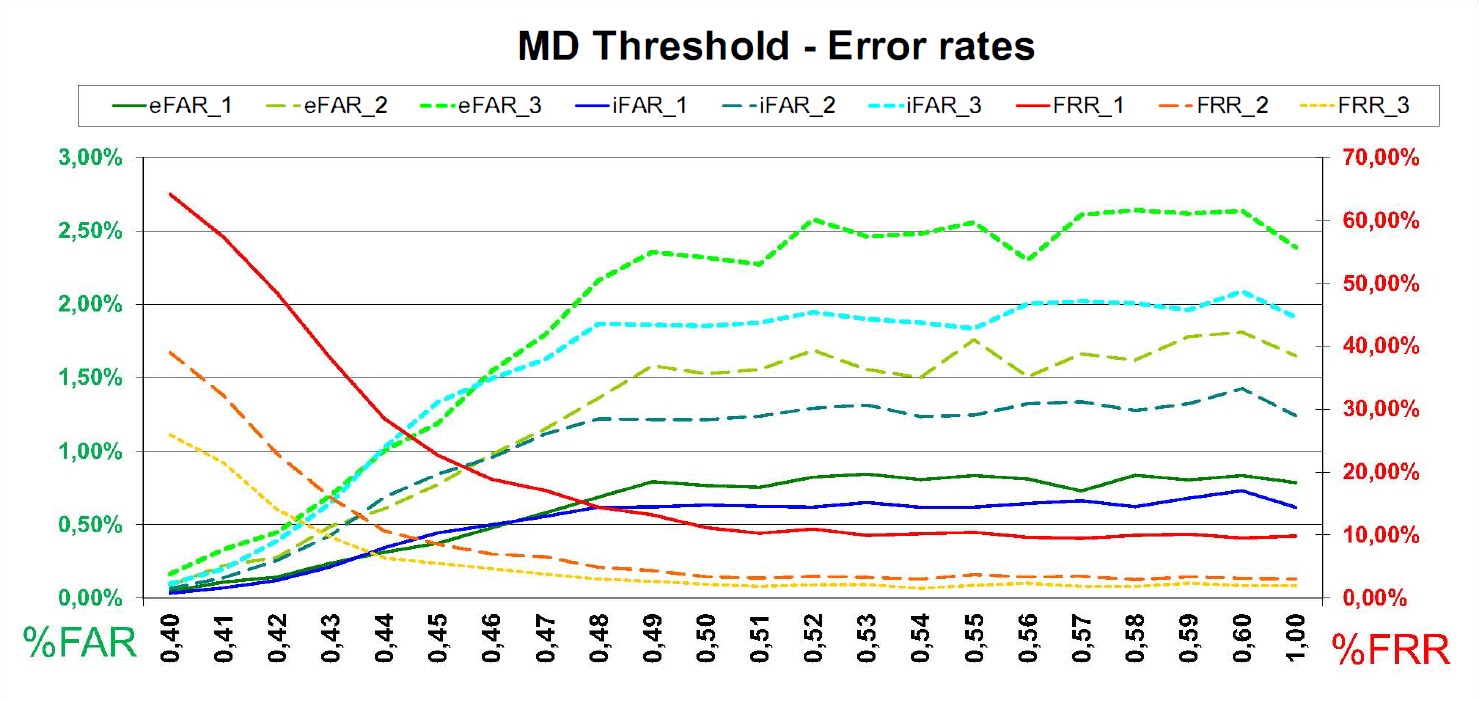
\includegraphics[width=0.7\textwidth]{messerman/messerman_thresh1}
    \caption{The distance threshold's effect on error rates as originally displayed in \cite{Messerman}. The scales for FMR and FNMR are on the left and right side of the graph, respectively.}
    \label{fig:messerman-threshold}
\end{figure}

The authors report the PA system's performance by using FAR and FRR, however they distinguish \textit{internal} FAR (iFAR) from \textit{external} FAR (eFAR), depending on whether the attackers are other legal users of the application or unknown adversaries.
As these rates are for the algorithm level, I will hereby use the terms FMR and FNMR as a correction.
A factor that had a significant impact on these rates was the maximum distance (MD) threshold, as seen in \cref{fig:messerman-threshold}.
The authors further separated each error rate into three rates corresponding to how many samples of 50 keystrokes were run through the classification algorithm before a final decision was made.
They refer to these runs as \textit{trials}, and they tested the system for 1, 2, and 3 trials.
For example, "eFAR\_2" represents the external FMR when the final decision is based on two trials. 

As \cref{fig:messerman-threshold} shows, the internal and external FMRs were negatively affected by increasing the number of trials, while the effect on FNMR was positive.
More imposters escape detection as they are given more chances per probe, and genuine users are less often wrongfully rejected.
Though both rates are affected, the number of trials affects the FNMR on a much larger scale than the FMRs.
As an example, for a distance threshold of 0.46, the difference in FNMR between one and three trials is slightly more than 10\%, while the difference in FMR is around 1\%.

%\begin{figure}[h]
%    \centering
%    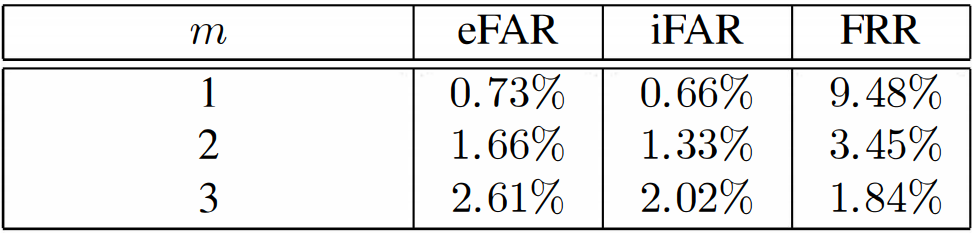
\includegraphics[width=0.4\textwidth]{messerman/messerman-perf2}
%    \caption{The results of the experiments in terms of iFMR, eFMR, FMR for \textit{m} trials per decision, with a maximum distance threshold of 0.57. \cite{Messerman}}
%    \label{fig:messerman-perf}
%\end{figure}

\begin{table}[h]
    \centering
    \begin{tabular}{lllllll}
         \bf Trials & \bf eFMR & \bf iFMR & \bf ANIA & \bf FNMR & \bf ANGA\\
         1 & 0.73\% & 0.66\% & 50-150 & 9.48\% & 527--1582 \\
         2 & 1.66\% & 1.33\% & 50-150 & 3.45\% & 1449--4347\\
         3 & 2.61\% & 2.02\% & 50-150 & 1.84\% & 2717--8152\\
    \end{tabular}
    \caption{Performance of the experiment in terms of error rates for \textit{m} trials per decision, with a maximum distance threshold of 0.57 as presented in \cite{Messerman}. ANIA and ANGA columns are added added by me.}
    \label{tab:messerman-perf}
\end{table}

\cref{tab:messerman-perf} shows the overall performance of their PA system.
As the block length varies between 50--150, the real ANIA and ANGA is impossible to calculate.
However, the authors state that they found an average of 32 shared n-graphs when the block length was 50 and stored samples of length 700, which implies that 50 keystrokes is often enough to perform an authentication.
Therefore, the real ANIA and ANGA are likely around the lower values in the table.

Finally, the authors report an average computation time of 409--554ms per decision on a 1 GHz Pentium 3 processor. 
Compared to Gunetti and Picardi's 140 seconds, this is clearly an improvement, however the fact that a decision is made every 50-150 keystrokes as opposed to 800 must be taken into consideration.

\section{Discussion}
The proposed PA system provides remedies for some of the issues in \cite{gnp}.
One of said issues was the large block size of 800, which has been reduced to 50-150 in \cite{Messerman}.
In terms of ANIA rates, this is a great improvement, as imposters are on average detected after 50-150 keystrokes only.
However, the ANGA rates are also lowered, causing genuine users to be locked out on average after 2717-8152 keystrokes in the best scenario (3 trials).
Compared to Gunetti and Picardi's ANGA of over 16000 keystrokes, this is an obvious downgrade.
Still, considering that the target system is an e-mail application, this would in many cases not result in many lockouts per day, since keystrokes outside of said application would not be recorded.

The proposed adaptive user model is a very interesting addition to the PA system.
Adapting to changes in the user's behavior is something that can have a positive impact on ANGA rates, leading to a better user experience as they are wrongfully locket out less often.
The user model is only updated if the result of a probe is a match.
However, imposters will in some cases be falsely accepted, causing the genuine user's profile to be corrupted with the imposter's typing patterns.
The authors mention that this can be prevented by limiting how many trials resulting in non-matches are allowed.
It seems like this could work in certain cases, but if the imposter has a sufficiently similar typing pattern to the genuine user and is accepted by one or more trials, the user profile is already corrupted and will give the imposter higher chances of being accepted in future authentication attempts.
Also, due to the way the authors described this prevention mechanism, it can be assumed that their system favors trials resulting in a match over those who do not.
This is not properly addressed in the article, but \cref{fig:messerman-threshold} supports this assumption, as a higher number of trials negatively affects FMR and positively affects FNMR.

\subsection{Scalability}
As similarly discussed in \cref{sec:gnp-scalability}, this system also has a reliance on other users in the application, though only a subset of the total userbase.
The addition of a threshold does however lower this reliance slightly, as it enables the system to perform better with very small userbases and also to function with only one single user.

On the issue of computation speed, the half second response time is more suitable for my master thesis than the 140 seconds in \cite{gnp}.
Even so, this does not necessarily mean that I can use this PA system as a whole, as there are a number of problems to be discussed.

\subsection{Enrollment}
Due to how the authors conducted their experiments, the reported performance is subject to discussion.
Only 3500 keystrokes were needed to build a user profile ready to be used for authentication, which is very efficient both for the length of the enrolment process, as well as for scalability in terms of storage.
Compared to Gunetti and Picardi's user profiles based on $14*800\approx{11200}$ keystrokes \cite{gnp}, a minimum of 3500 is a better fit for an online e-mail application.
The low block size of 50--150 also greatly limits the damage potential for imposters.
If this PA system were to be used for securing an entire operating system though, such as the setting in my master thesis, the experiments in both research articles \cite{gnp, Messerman} are unsatisfactory in captured variance of behavior.
Messerman et al.'s \cite{Messerman} experiments probably captured higher variance, as there was no restriction to language used, and the volunteers were not suggested to write about any certain topics.
As the keystrokes were recorded in the background, the participants were not merely typing text in order to produce samples; they were simply composing e-mails that they otherwise would have written regardless of participating in the experiment.
Still, restricting to only e-mails means other behavior such as gaming and coding was not recorded. 
It is not known how this system would perform in such scenarios with only 3500 keystrokes being covered.

\subsection{Performance evaluation issues}
When evaluating the performance of the PA system, the authors used various settings and parameters, as already mentioned in \cref{sec:messerman-experimental}.
When evaluating different performance metrics, they included specific settings in footnotes.
Examples of this are the experiments for investigating how the performance was affected by the total number of users in the userbase as well as the number of users considered in the decision process.
In both of these cases, they used 17 external imposters and 23 internal imposters/legitimate users.
This is a total of 40 users, which fits the number of users producing over 3500 keystrokes: $55-15=40$.
Apart from this, they also showed the settings for investigating the maximum distance threshold's impact on error rates, which is the experiment shown in \cref{fig:messerman-threshold}.
Here they used 20 external imposters and 30 internal imposters/legitimate users.
As this puts the total involved users as 50, they seem to contradict their own minimum number of keystrokes in the enrollment process.
The true performance results are therefore not completely clear, as they do not explain this contradiction in their article.

Another issue regarding their performance evaluation is the fact that the results in \cref{tab:messerman-perf} are achieved with a maximum distance threshold of 0.57.
Again, the authors do not explain the reasoning for this specific value.
This leads me to believe that the results are influenced by overfitting, as 0.57 happens to be an optimal threshold as seen in \cref{fig:messerman-threshold}, especially regarding external FMR for 1 trial, which shows a valley at that threshold.
If the authors indeed overfitted their experiment to their dataset, it is difficult to imagine the true performance of the PA system employed in practice.

Lastly, I would like to mention two unclear issues, with the first being the lack of clarity regarding which n-graphs were considered in the experiments.
They do mention that they found an average of 32 shared digraphs between attempt samples of 50 keystrokes and stored samples of 700 keystrokes, however they do not tie this up to the performance evaluations.
Secondly, they do not explain why they only use the R-measure, as opposed to combining it with an A-measure as Gunetti and Picardi did \cite{gnp}.
Seeing performance results for a combined R and A distance would be interesting, both for the effects on error rates and computation speed.

\chapter{Ferreira and Santos}
\label{chap:ferreira}
Another PA system based on Gunetti and Picardi's work was published by Ferreira and Santos in 2012 \cite{superResults}.
They use a block size of 250 keystrokes and also periodically update the user profile after three successfully authenticated attempts, in other words by merging the attempts into a sample of 750 keystrokes to be integrated into the user profile.
While they state that one such sample technically is enough to start the authentication stage, the accuracy would obviously be negatively affected by having such a small user profile.
The user profile contains 15 such samples, and during authentication these are \textbf{merged} to one template based on $15*750 = 11250$ keystrokes to be compared to the 250 keystroke attempt sample. 
As new 750 keystroke samples are submitted, the oldest ones in the user profile are replaced by the new samples, not unlike the adaptive user model in Messerman et al.'s PA system \cite{Messerman}.
An important difference between the two systems is that while Messerman et al. only uses the R measure, Ferreira and Santos' system utilizes both R and A measures for distance calculations.
%As opposed to the PA system proposed by Messerman et al. \cite{Messerman} which was discussed in \autoref{chap:messerman}, Ferreira and Santos' system uses both R and A measures for their distance calculations.

They refer to a previous study \cite{superOld}, where they along with a third author describe their own method for calculating A measures.
As shown in \cref{sec:gnp-algorithm}, Gunetti and Picardi used a threshold of 1.25 in the calculation of A measures to determine whether n-graphs from the probe and reference were similar.
Ferreira and Santos' method takes advantage of standard deviations, as every n-graph of a \textit{subtemplate} has an associated average, standard deviation and number of occurrences.
Subtemplates (called subsamples in original paper) are separated collections of \textbf{dwell times} for single keys, \textbf{flight times} for digraphs and \textbf{down-down latencies} for di-, tri- and fourgraphs extracted from a sample.

An example of a subtemplate would be all trigraph latencies extracted from a sample.
Then, every trigraph in the subtemplate would have a standard deviation, average latency and number of occurrences within the subtemplate.
Using these values, they calculate the 10\% most consistent n-graphs in every subtemplate, and store a record of them in the user profile.
During comparisons, they apply a lower similarity threshold when comparing n-graphs that are among the 10\% most consistent.
This enables them to place more strict expectations where the genuine user rarely deviates from their usual typing patterns.
They mention that they by default use a similarity threshold of 1.10 for consistent n-graphs and 1.25 for others, and that these are adjusted based on every individual user's timing consistency \cite{superOld}.
Unfortunately, they do not describe exactly how this adjustment is performed.

Taking consistent n-graphs into account, the rest of the A measure is calculated as described in \cref{chap:gnp}. The R measure is also calculated in the same manner as the original method, and the A and R measure are combined into what they call the \textit{global score}.
Note that I will refer to their matching score as a \textit{distance} in order to more easily show their system's relation to the other PA systems using R and A measures. 
Distances and match scores generally work in the same way, except high scores indicate more similarity, whereas high distances indicate \textit{dissimilarity}.
While a probe is compared to several other users in \cite{gnp, Messerman}, Ferreira and Santos' PA system bases its decisions solely on a global distance threshold.
Interestingly, the global distance threshold is calculated individually for every user.
This is done computing the global distance between every 750 keystroke sample in the database and the merged references, not including their own occurrences, which essentially is a leave-one-out cross validation.
The average distance of all of these calculations give an expectation of how the genuine user should be performing compared to their own profile.
The global distance threshold is then set to this average distance minus a static degree of tolerance in order to allow for some variations.
This threshold largely affects the error rates, and can be changed to balance FMR and FNMR according to how strict the system should be.
This is further shown in \cref{sec:ferreira-experiment}.

Another interesting feature that the authors proposed is to asynchronously authenticate the user when certain events happen.
One example could be after a longer period of silence where the genuine user may have left the workstation, an authentication could be triggered after 75 keystrokes.
Then, a sample consisting of the last $175 + 75 = 250$ keystrokes would be tested, in order to potentially catch an imposter who would have taken control of the computer.
Attempting to save or overwrite important files could also trigger this functionality.
The example of 75 keystrokes may be too small to weigh down the 175 genuine keystrokes in a real scenario, though an experiment could be performed in order to optimize the ratio.
Also, this kind of asynchronous authentication could in practice be implemented in any PA system, but it is rarely mentioned in literature as a possible option.

\section{Experimental setting}
\label{sec:ferreira-experiment}
60 participants installed a logging software on their computers which captured their keystroke data in the background, never interfering with their daily activities.
The data collection period lasted for two weeks and 15 samples were collected to build user profiles in addition to another 15 samples which were to be used for testing.
These extra samples were used both to simulate genuine access attempts and as imposter attempts, resulting in a total of 900 genuine attempts and 53100 imposter attempts \cite{superResults}.


\begin{figure}[h]
    \centering
    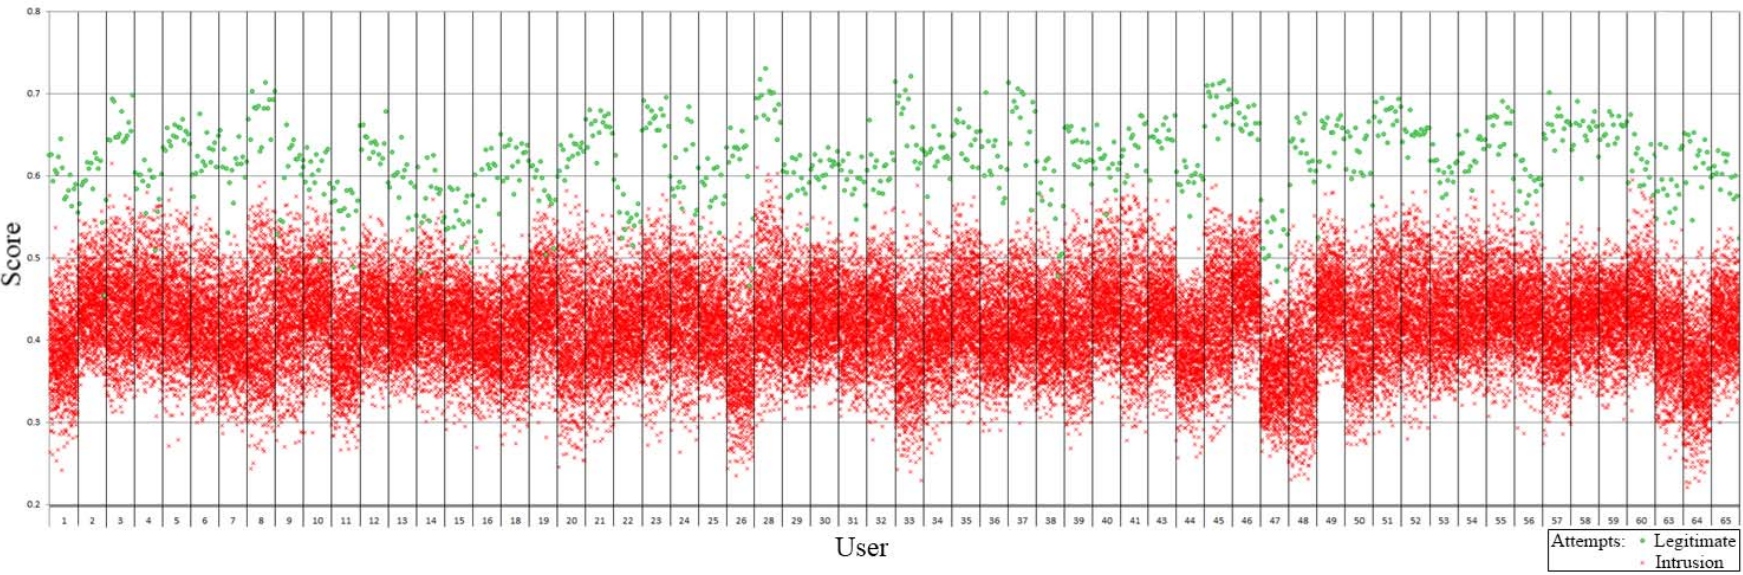
\includegraphics[width=1\textwidth]{ferreira/distr}
    \caption{Distribution of scores for genuine and imposter attempts against all user profiles as presented in \cite{superResults}.}
    \label{fig:ferreira-distr}
\end{figure}

The results of the simulations showed an equal error rate of 1.4\%, and they point out a specific setting for the degree of tolerance mentioned earlier which gives a 0.5\% FMR and 2.7\% FNMR.
This translates to an ANIA of $250 / (1-0.005) \approx{251}$, and ANGA of $250 / 0.027  \approx{9259}$, which will be discussed in \cref{sec:ferreira-discussion}.
They also found that there was a clear distinction between genuine and imposter attempts as seen in \cref{fig:ferreira-distr}, though if the authors used a distance metric as opposed to a score, the red and green dots in the figure would swap places. 

While some of the users generally have lower scores to their own profiles, the imposters score even worse, indicating that having custom distance thresholds for every user benefits the performance of the overall system.
I would like to mention that it is unclear why the figure involves 65 users instead of 60.

The authors also created a prototype of the PA system for testing it in real time, though at a smaller scale than the simulations.
Ten participants each produced a fixed-text stored sample of 200 keystrokes, and testing was conducted by having one genuine attempt and a random person acting as an impostor. This was done in 200 iterations, and resulted in a 0.5\% FMR and a 5.5\% FNMR, which shows that the smaller sample size negatively affected the FNMR, and thus also affected the ANGA which in this case was 3636.

\section{Discussion}
\label{sec:ferreira-discussion}
Ferreira and Santos' PA system seems particularly fitting for my master thesis, as its intention to be used for protecting an entire workstation by observing keyboard input in all applications and contexts is similar to that of Mondal's CA system which I will be extending \cite{mondal}.
The experiment's unconstrained data collection phase also matches Mondal's experiment quite well, which makes comparing the systems more sensible.
As I will be using Mondal's database for my own project, I am likely to receive similar results when applying Ferreira and Santos' methods to it, as the data should have similar amounts of variation in typing behavior per user.

While their method for asynchronous authentication is a great measure for possibly detecting imposters even earlier than the block size originally allows, and even on special triggers, this is mostly relevant for actual real-time implementations of the software.
% Omitted by suggestion: My master thesis will revolve around simulations and analysis, and I could therefore omit this functionality if I were to integrate this PA system into the CA system.
Mondal's CA system already tries to detect imposters as early as possible, and for that reason partly eliminates the need for the proposed asynchronous authentication.

\subsection{Classification}
A great feature of the PA system is its sole reliance on a user-fitted global distance threshold.
Not only does this ensure that users who tend to score poorly against their own user profile still can use the PA system with satisfying performance, but it also lets the system avoid involving other users in the classification process.
As the PA system operates application-wide, one can imagine a scenario where college campus computers would install the PA system.
Such computers are accessible by thousands of students, and comparing the typing patterns of one user to every other registered student such as Gunetti and Picardi's original system would do \cite{gnp} is clearly not practical.
While Messerman et al. \cite{Messerman} would not show the same scalability issues due to only including a subset of all students, Ferreira and Santos' system inherently avoids the potential problem of having a genuine user falsely rejected due to their probe haphazardly being more similar to another student's behavior than that of their own.

While not involving other users positively affects the scalability of the PA system, the rather large user profiles consisting of over 11000 keystrokes could pose a challenge in real-time applications if they have a very large amount of users.
This could probably be reduced if necessary, though the performance impact would have to be analyzed extensively beforehand.
%Omitted by suggestion: Regardless, as I will not make a real-time application this is not an issue in my specific case.
Another feature that could be problematic for a real-time implementation is periodically updating the user profile, as it would corrupt the user database if imposters were falsely accepted.
However, three consecutive attempts would have to be accepted in Ferreira and Santos' system, which lowers this risk.
If an imposter were accepted three times in a row, the user profile would have to be retroactively rolled back to a valid state.
Again, this is another feature that can be omitted from the simulations in my master thesis.

\subsection{Performance}
Seen in relation to the short block size and high variance datasets, achieving an EER of 1,4\% is remarkable.
An imposter's window of opportunity is considerably smaller with a block size of 250 keystrokes, compared to Gunetti and Picardi's 800 block size.
A block size this small is also very suitable for integration with the CA system, as the CA's ANIA rating is around 500 \cite{mondal} at its best settings.
This means that the PA system could positively affect the ANIA rating, as periodic authentications would occur every 250 keystrokes.

As the static (system specific) degree of tolerance can be changed to influence the relationship between the FMR and FNMR, this allows for tailoring the level of strictness of the PA to better match that of the CA.
However, I would have to be aware of the possibility of overfitting the degree of tolerance to Mondal's dataset.
A preventive measure could be to select a random subset of the users and adjusting the degree of tolerance to fit the subset, and using that degree of tolerance for the entire dataset, similarly to the method described in \cref{chap:gnp}.

Regarding the performance results from the \textit{prototype} experiment, it does give some indication that the system could work in real life, though as the context was highly controlled with static text and relatively few participants, not too much emphasis can be put those results compared to those of the main experiment.


%Positive: Gives ROC curve. Prevents us from only seeing overfitted performance evaulations.


%Negative: Doesn't mention computation time. Though, it should not be high at all, as probes are only compared to genuine user profile.
\subsection{Follow-up study}
A follow up study was performed by Santos and two other authors where they investigated ways to lower the sample size and positively affect the performance of the PA system \cite{Pinto2014}.
Using different weights for different types of features (dwell, flight, digraph, trigraph, fourgraph) and different weights for A and R measures, they were able to reduce the size of attempt samples to 150 keystrokes, with an FMR and FNMR of around 2\%.
They found that dwell times, flight times and digraphs latencies were the most effective features to be used for authentication.
However, the experiments were performed with only 10 participants, and generally lacks clarity, especially so regarding the performance.
I will therefore not discuss this paper in detail.


\chapter{Ahmed and Traore}
\label{chap:ahmed}

The PA system previously discussed in dedicated chapters have all applied a statistical approach for their authentication schemes.
Machine learning is another approach that has gained popularity in recent years, and Ahmed and Traore \cite{Ahmed}'s proposed PA system is based on this approach.
One of their goals was to decrease the needed amount of keystroke data from enrollment.
PA systems which rely on an unconstrained free-text enrollment phase will, depending on the amount of data collected, have varying amounts of different n-graphs recorded and stored.
Therefore, a user may generate an attempt sample containing one or more n-graphs not present in the reference.
For this reason, the authors proposed a method called \textit{sorted time mapping} for predicting what timing features a missing n-graph would have, based on relations between the n-graphs present in the reference.

Their system relies on covering the most frequently used \textit{monographs}.
The definition of "frequent" in this context is flexible, as it means the set of keys with a higher chance of occurrence than a certain probability threshold.
In this case, "chance of occurrence" means the chance of a key being \textit{the next key to be pressed}, not the chance of it occurring once in an entire enrollment sample.
The size of the enrollment sample must then be decided so that all monographs above the probability threshold are covered.
For instance, if the probability threshold is set to 0.001, all keys with higher chance of occurrence than 0.1\% must be covered in the enrollment sample, and the size of the enrollment sample must be set to a value that satisfies this criteria.
More on how this size is determined is described in \cref{sec:ahmed-experimental}.

\section{Neural networks}
Two feed forward neural networks of type multilayer perceptron (MLP) are trained during using the enrollment sample and used for behavior modeling.
One network processes monographs, while the other processes digraphs.
For training the digraph network, a \textit{digraph mapping table} must be generated based on the data from the enrollment sample.
This table contains an entry for the keycode of every key in the enrollment sample.
These entries are sorted by the average flight time \underline{to} the monographs, based on all recorded digraphs with that monograph as the second key.
Every key then has a \textit{digraph key order (DKO)}, which represents the average flight time to that key relative to all other keys. 
The actual average flight times are excluded from the table; only the DKO of each key is included.
One may notice a certain resemblance to the calculation of Gunetti and Picardi's \cite{gnp} R measure.
Similarly, a \textit{monograph mapping table} is needed for training the monograph network. 
This table is ordered by dwell times instead of flight times, giving each key from enrollment a \textit{monograph key order (MKO)}.

The digraph network is trained with all digraphs from the enrollment sample encoded as DKOs.
As seen in \cref{fig:ahmed-networks} (b), it is trained with two inputs, namely "from" and "to", which are fed the DKO of the two keys involved in a digraph. 
The training output is the actual flight time of the digraph.
Training the monograph network is done similarly, though with MKOs as input and actual dwell times as output.
Both networks are trained using the Levenberg–Marquardt \cite{levenberg_1944} algorithm and the monograph network's hidden layer consists of 16 nodes, while the digraph network's hidden layer has 40.

\begin{figure}[h]
    \centering
    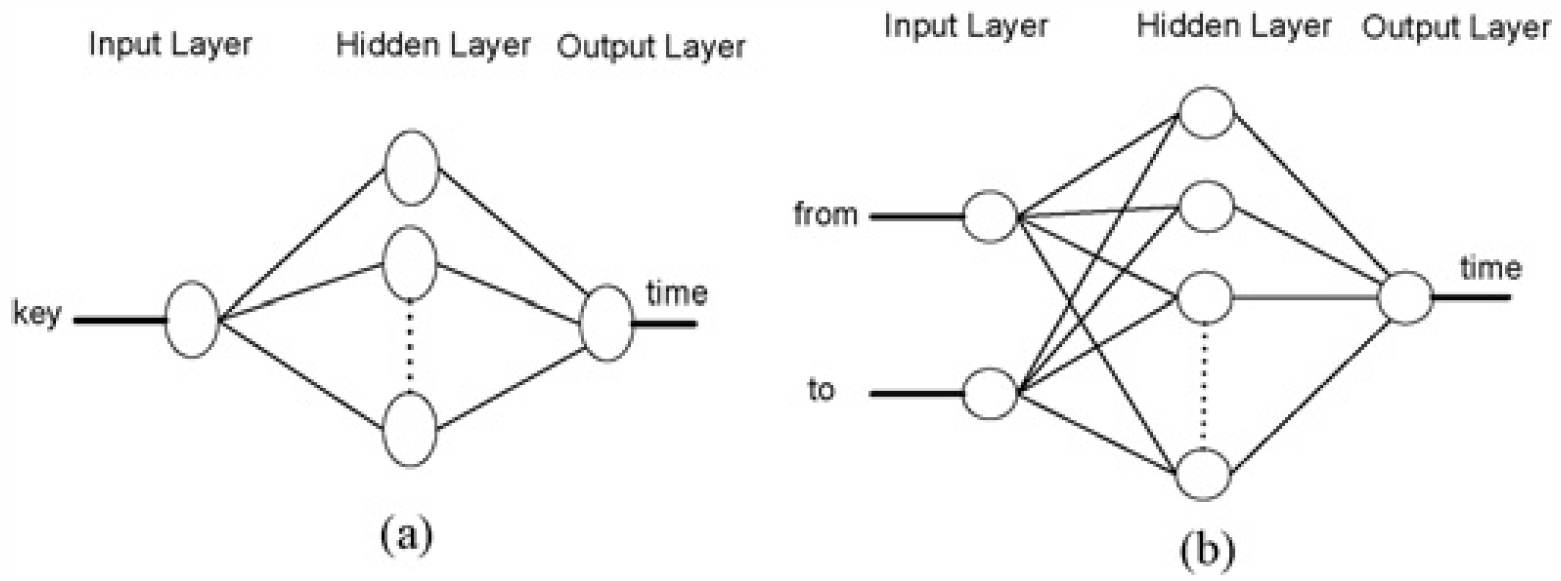
\includegraphics[width=0.75\textwidth]{ahmed/networks}
    \caption{The structure of the monograph network (a) and digraph network (b), as presented in \cite{Ahmed}.}
    \label{fig:ahmed-networks}
\end{figure}

When the neural networks are trained, their weights are stored along with the monograph and digraph mapping tables as a \textit{reference signature}.
The reference signature is loaded during the authentication phase, as all users of the PA system utilize the same two neural networks, only with their own mapping tables and network weights.
\Cref{fig:ahmed-authentication} shows how data is processed during periodic authentication.
\begin{figure}[h]
    \centering
    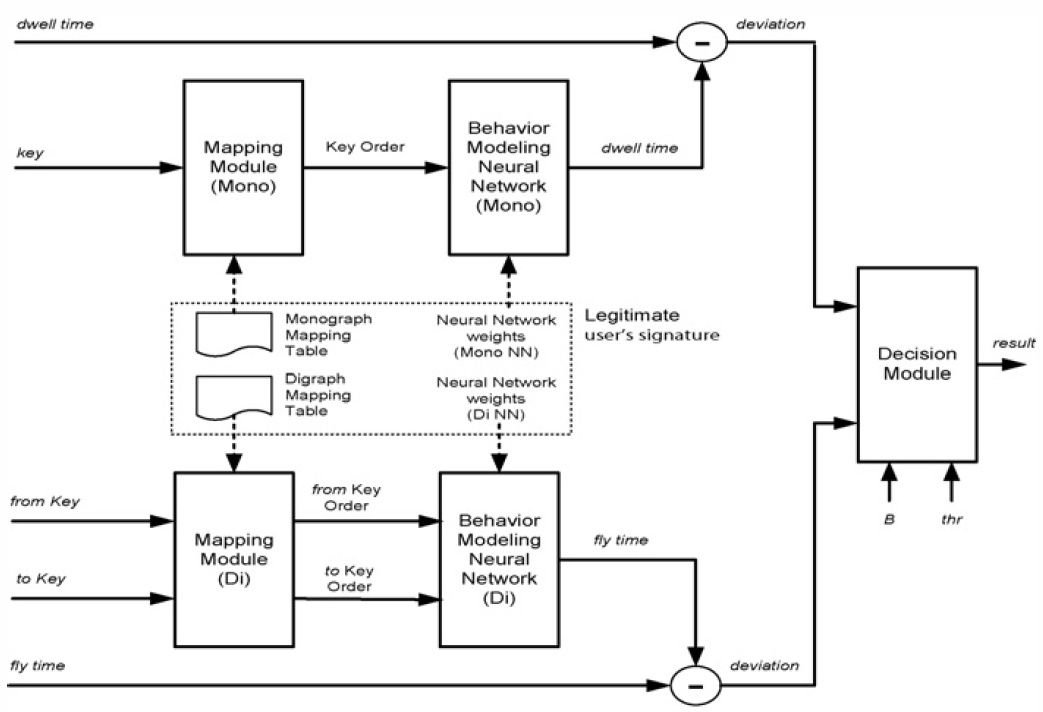
\includegraphics[width=0.75\textwidth]{ahmed/authentication}
    \caption{Ahmed and Traore's periodic authentication mechanism \cite{Ahmed}.}
    \label{fig:ahmed-authentication}
\end{figure}
When an attempt sample is collected, monograph dwell times and digraph flight times are extracted from the raw data, essentially acting as probes.
Recorded monographs are mapped into MKOs using the genuine user's monograph mapping table.
The MKOs are then fed as input to the monograph network which is loaded with the genuine user's weights.
The output dwell times represent the expected values which are compared to the dwell times from the attempt samples, with each comparison resulting in a deviation.
When all dwell time deviations are fed to the decision module, it calculates the average absolute deviation (AAD), using the following equation \cite{Ahmed}:
\begin{equation}
AAD\textsubscript{mono}={{\sum\limits_{i=1}^{N_{\rm mono}}{{{\left\vert{d_{i}-D_{i}}\right\vert}\over{D_{i}}}\times100}}\over{N_{\rm mono}}}
\end{equation}
with N\textsubscript{mono} being the total number of monographs from the probe, d\textsubscript{i} being the \textit{i}th probe monograph's dwell time and D\textsubscript{i} being the \textsubscript{i}th monographs's expected dwell time.
The expected dwell time is the output of the monograph network.

Digraphs are processed similarly, as seen in \cref{fig:ahmed-authentication}, though the digraph network outputs an estimated flight time if the current digraph being processed was not included in the training.
It calculates this estimated flight time by viewing the digraphs relation to the other digraphs based on the DKOs from the digraph mapping table.
The actual flight time of the probe digraph is compared to the output of the digraph network, regardless if the digraph was missing from enrollment or not.

When the AADs for mono- and digraphs (AAD\textsubscript{di}) are calculated, the decision module combines them linearly using weights.
The combined deviation is calculated using the following equation:
\begin{equation}
D = B * AAD\textsubscript{mono} + (1-B) * AAD\textsubscript{di}
\end{equation}
where D is the combined deviation and B is a balancing factor (the authors vary between calling this a balancing, dependability and tuning factor).
The balancing factor is a value between 0 and 1, and lower values place more weight on the digraph AAD.
The final output is true or false, depending on the combined deviation and a selected decision threshold.
A combined deviation below the the threshold leads to the output being true, meaning the probe behavior is recognized as the genuine user.

\section{Experimental setting}
\label{sec:ahmed-experimental}
Their main experiment consisted of a completely unconstrained and uncontrolled collection phase, with 53 participants installing a keystroke logging tool on their personal computers.
They had a high variation in typing skills, age and gender, and around 18 000 keystrokes were collected from every user on average over the course of five months.

As mentioned earlier, the size to be used for enrollment samples must cover the most frequently used keys.
During the experiment, the authors investigated how many keystrokes were needed for a probability threshold of 0.001, which corresponded to the 60 most frequently used keys \cite{Ahmed}.
They found that 1350 keystrokes were needed to cover 100\% of the most frequently used keys for three arbitrary participants, and decided that 1500 keystrokes would be used as an enrollment sample size for the rest of the experiment.

The first 1500 keystrokes from the experiment's collection phase were used to build the user profile, consisting of mono- and digraph mapping tables, along with networks with user specific weights.
The rest of the keystrokes collected were divided into attempt samples of length 500, each being used as a genuine test sample and for attacking all other users.
% They call this a leave-one-out cross-validation test (LOOCV), though it seems to me that this is not the case as they specifically state that the user profiles were built using the \underline{first 1500} keystrokes \cite{Ahmed}.
%This means that all test sets are tested against the same training set, which can not be called cross-validation.
The test was repeated for all 53 participants.

\subsection{Performance}
\label{sec:ahmed-performance}
When using attempt samples of length 500 and balancing the mono- and digraphs equally, they achieved an EER of 2.13\%.
Varying the decision threshold allowed for tuning the relationship between FMR and FNMR, and the authors point at a specific threshold level of 77\% which gave an FMR of 0.0152\% and FNMR of 4.82\%.
This corresponds to an ANIA of 500, and ANGA of $500 / 0.0482 = 10373$.
The experiment's receiver operating curve (ROC) can be seen in \cref{fig:ahmed-withdi}, where different threshold levels are marked with an X.
The authors also tested the performance without digraph predictions, where every digraph missing from the user profile was ignored.
This resulted in a worse performance, and judging from \cref{fig:ahmed-withoutdi}, the equal error rate seems to be around 12\%.

\begin{figure}[!tbp]
  \begin{subfigure}[b]{0.5\textwidth}
    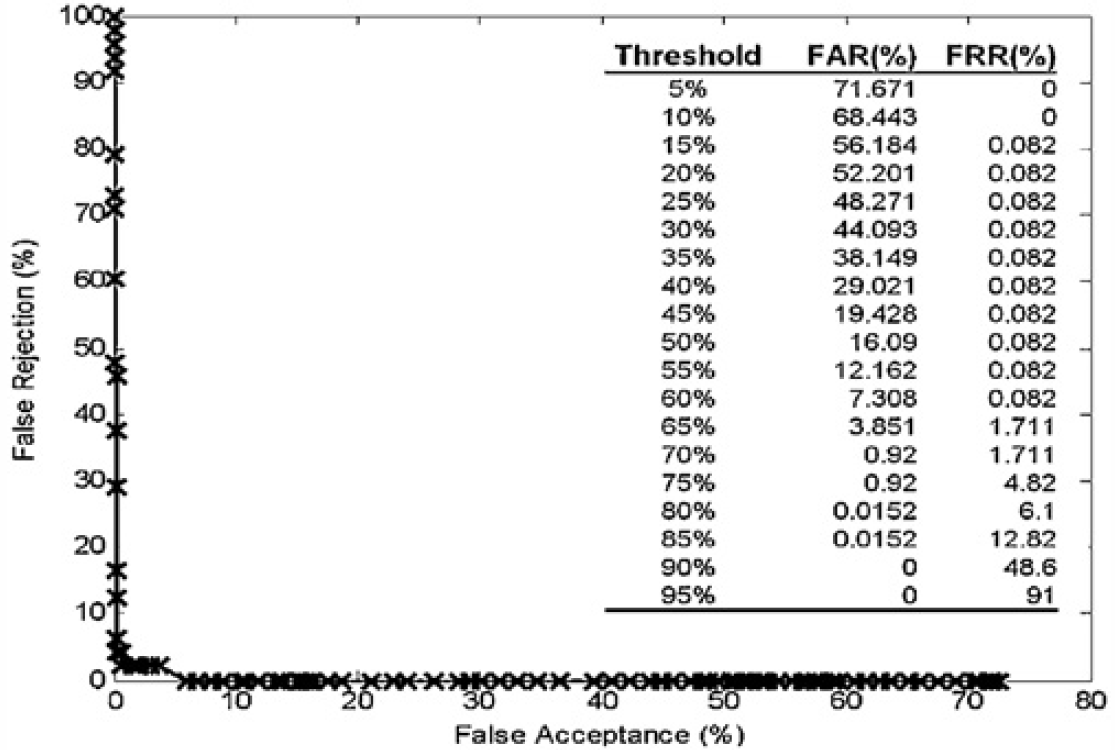
\includegraphics[width=\textwidth]{ahmed/roc}
    \caption{With digraph prediction.}
    \label{fig:ahmed-withdi}
  \end{subfigure}
  \hfill
  \begin{subfigure}[b]{0.5\textwidth}
    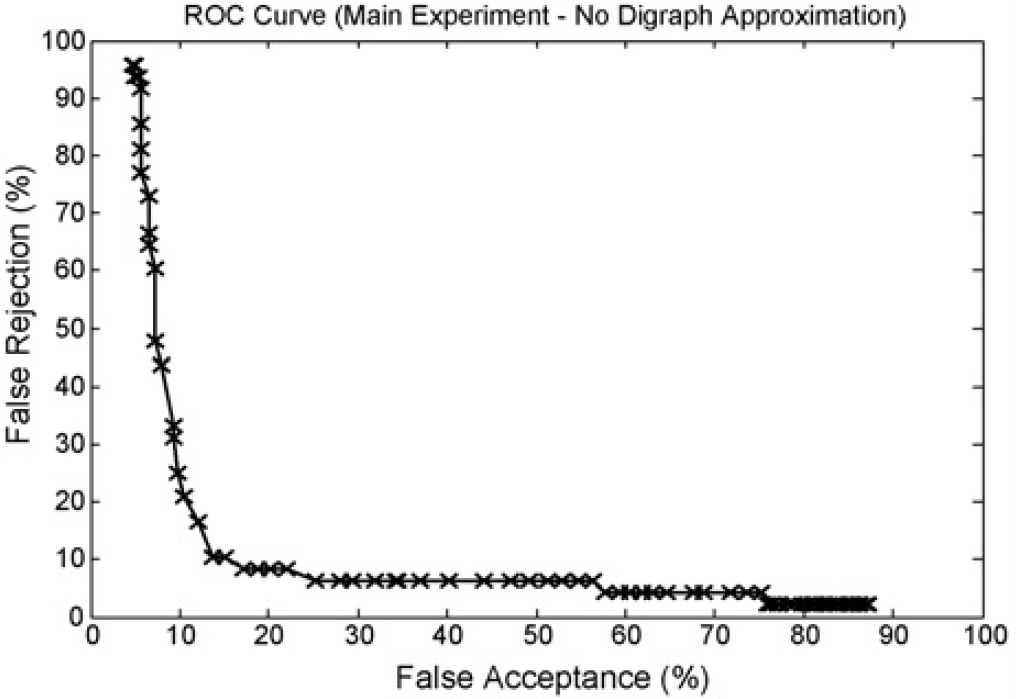
\includegraphics[width=\textwidth]{ahmed/without-di}
    \caption{Without digraph prediction.}
    \label{fig:ahmed-withoutdi}
  \end{subfigure}
  \caption{Receiver operating characteristic curves of the performance in terms of FMR and FNMR with and without digraph prediction \cite{Ahmed}.}
\end{figure}

\section{Discussion}
\label{sec:ahmed-discussion}

\subsection{Sample sizes}
\label{sec:ahmed-discussion-sample}
At a first glance, a block length of 500 keystrokes seems rather lengthy, especially compared to the block lengths of Messerman et al. \cite{Messerman} and Ferreira \& Santos \cite{superResults}.
Even so, it could still positively impact of Mondal's \cite{mondal} CA system, as that system has an ANIA of around 500 keystrokes and above, depending on the classification method used.
As that is an \textit{average} number of imposter actions, it implies that some imposters are not detected until more actions are performed.
Some may not be detected at all, and therefore, incorporating a PA system with a block length of 500 could in many cases help lowering the CA system's ANIA rate.

The enrollment sample size of 1500 keystrokes is impressive, and their digraph prediction functionality is what enables the PA system to rely on such small amounts of information being present in the user profile.
The method for deciding the size of enrollment samples does raise a concern though, as they based the decision on how many keystrokes were needed to cover 100\% of the most frequently used keys, in their case specifically for the probability threshold of 0.001.
It seems that if another probability threshold is to be used, anyone implementing this PA system must investigate the sample size needed to fit their own probability threshold. 
If true, this means that an experimental collection phase has to be performed prior to implementing the PA system and using it.

While only needing 1500 keystrokes to enroll a user allows for quickly initiating the authentication stage, the varying contexts covered in enrollment inherently suffers, which is another concern.
Considering that a PA system targeting application-wide monitoring needs to take into account behaviors such as playing various games, writing text and other contexts, such a short enrollment phase may only cover a subset of the needed information.
It would be useful to see the error rates for gaming behavior in the authors' experiments.
Unfortunately, this information is not provided.

It is also worth mentioning that the authors were inconsistent in their description on sample sizes, varying between using keystrokes and digraphs as a measure of sample length.
1500 keystrokes and 1500 digraphs does not represent the same length, as 1500 keystrokes will at best contain 1499 digraphs.
Also, two keystrokes with a very long flight time between them cannot truly be considered a digraph as this generally means the user paused their typing. 
This means that for every such pause, more keystrokes are needed to cover 1500 digraphs, further distancing the "keystrokes" and "digraphs" measures of length.
In my description of their system, I have used "keystrokes" as a measure of length, based on the assumption that this is what they mean.

\subsection{Experimental settings}
Similarly to the PA system discussed in \cref{chap:ferreira}, the collection phase matches that of Mondal's \cite{mondal} experiments, as it was unconstrained and performed on the participants' own computers.
As they also had a high variance in participant characteristics such as age and gender, their dataset should include a rather large spectrum of contexts.
This means that the test probes generated should cover those different contexts even if only 1500 keystrokes were used for enrollment, which partly covers the issue mentioned in \cref{sec:ahmed-discussion-sample}.

The fact that they used the \textit{first} 1500 keystrokes for building user profiles in an unconstrained collection phase seems slightly counterintuitive.
Immediately after a user installs the keystroke monitoring software is probably a period of time where they are more conscious about the fact that their typing patterns are being collected. 
This could lead to some tension which could lead to slight variations representing uncharacteristic behavior.
Extracting keystrokes slightly further into the collection phase could therefore be a viable alternative.
The keystrokes from the first part could then be used for testing instead, or possibly even ignored.

%Positive: high variation in collection. Very old computers though (probably old dataset), but that doesnt necessarily mean anything.

\subsection{Neural networks}
The neural networks in the PA system output expected timing values for mono- and digraphs, as opposed to making the decision themselves.
The final decision is made based on deviations alone, and the PA system is therefore only reliant on genuine user data for training.
This removes the need for shipping the software with imposter data.
However, the dataset used to test Mondal's \cite{mondal} CA system does have available imposter anyway, so this does not have a meaningful impact for incorporating the PA system into said CA system.

Kim et al. \cite{KIM2017} mentioned that Ahmed and Traore's system is impractical due to high amounts of network weights to be optimized seen in relation to the amount of available training data.
Abo-alian et al. \cite{CPE3718} also criticized the solution for it's small sample size and scalability issues.
While it may be true, it seems unfair as the purpose of Ahmed and Traore's work was indeed to reduce the size of enrollment samples.
Scaling the system into much larger sample sizes seems to defeat the purpose of picking the system over others in the first place.

Ahmed and Traore \cite{Ahmed} claim that their system has a far lower processing time compared to the state of the art, with Gunetti and Picardi \cite{gnp} being mentioned in that context.
Unfortunately, they only specify the time needed to train the neural networks, which was below two seconds for both networks on a 2.8 GHz processor.
In case the user profile needs to be updated, this should be fast enough to be done in periods of inactivity.
That aside, the processing time for the neural networks is likely to be negligible.

%Negative: Must be retrained
%Negative: They claim "far lower processing time" than 

%Can possibly use the digraph approx. method along with another system?



% http://onlinelibrary.wiley.com/doi/10.1002/cpe.3718/full WRITE ABOUT THIS AFTER AHMED



% http://ieeexplore.ieee.org/document/7529146/ this one seems pretty good (state?)
%NOTE: SLIDING? \cite{sliding}. Probably worth writing about (incl. in state)
%NOTE: VILLANI MAY BE WORTH INCLUDING BECAUSE OF EUCLIDIAN DISTANCE (incl. state)
% https://www.hindawi.com/journals/tswj/2013/408280/talks about machine learning
\chapter{Concluding discussion}
\label{chap:conclusion}

After having covered the state of the art and reviewed a number of PA system in detail, various mechanisms and algorithms have been discussed.
As stated in \cref{chap:introduction}, the systems have been reviewed as they are described in the original work.
However, for incorporating a PA system into a CA system, parts of different PA systems can be mixed and optimized to fit the original CA system.
Therefore, certain aspects I have criticized may be excluded from the resulting CA+PA combination so that their disadvantages can be avoided.
The excluded parts can then be replaced by more fitting functionality from other PA systems.

Gunetti and Picardi's \cite{gnp} R and A measures are a good representation of the state of the art for statistical approaches to PA, as they have been adopted by several other PA systems and give good results in terms of error rates.
Their original scalability problems have been addressed in a number of ways, including those discussed in \cref{chap:messerman} and \cref{chap:ferreira}, resulting in more practical systems.

Machine learning has also become a popular approach to PA, and the digraph prediction method presented by Ahmed and Traore \cite{Ahmed} allows a PA system to base itself on relatively small enrollment samples.
As Mondal's \cite{mondal} CA experiments were based on larger training data (around 5000 keystrokes) compared to that of Ahmed and Traore, it would be interesting to see how this functionality could interact with the CA system.
A possibility could be to have both the CA system itself and the incorporated PA system use the digraph prediction functionality, either in order to lower the amount of training data used, or to explore the effects on performance using the original amount. 
This needs further investigation.

One of the important focuses of this literature review has been on the block sizes, or the length of attempt samples.
Incorporating a PA system which bases itself on a block size much larger than the ANIA rate of the CA system would in many cases cause the CA system to detect imposters before the PA system could even gather enough information to make a decision.
This would essentially defeat the purpose of incorporating the PA system in the first place, meaning that block sizes smaller than or similar to the CA system's ANIA value is ideal.
That, in addition needing low a FNMR in order not to worsen the CA's ANGA rates is satisfied by the systems discussed in \cref{chap:messerman,chap:ferreira,chap:ahmed}.

The experiments performed to test the discussed PA systems also had similar data collection phases to that of the CA system's experiments, in the sense that they were based on free-text.
While the data collection in Messerman et al. \cite{Messerman} was done in an e-mail client and that of Gunetti and Picardi \cite{gnp} was done in a webform, Ferreira and Santos \cite{superResults} as well as Ahmed and Traore \cite{Ahmed} had completely unconstrained data collection phases.
This indicates that the PA performance rates may be similar on the CA system's dataset, further enhancing the confidence in parts of these systems being viable for incorporation into the CA system.

Lastly, I would like to mention that there may exist other potentially viable functionalities in existing literature outside of the reviewed PA systems.
An example of this is using a sliding window for attempt samples \cite{sliding}.
Instead of performing PA after every \textit{n} keystrokes where \textit{n} is equal to the block size used, the authentication can base itself on the same block size \textit{n}, but at more regular intervals.
This can be time based so that authentication is performed on a time interval, for instance one minute, using the last \textit{n} keystrokes recorded.
Of course, if the amount of keystrokes recorded since last authentication reaches \textit{n} before one minute has passed, the authentication would have to be triggered earlier.
Basing the sliding window on the amount of recorded keystrokes instead of time is also possible.
An example would be to execute the authentication after \textit{m} keystrokes where \textit{m} < block size \textit{n}.
Both of these cases allow the authentication to be performed more often than the block size alone would permit, possibly catching imposters more quickly.

This literature review has given me valuable knowledge, preparing me for my coming master thesis. This was the goal of the project, and though discussing every interesting PA system in detail was beyond the scope, the reviews in \cref{chap:gnp,chap:messerman,chap:ferreira,chap:ahmed} allowed me to perform a deep dive into a subset of the available literature.
Not only did this enhance my understanding of these specific PA systems, but allowed me to better understand the rest of the relevant literature.






% NOTE: Mention possibility of sliding window?


%NOTE: FIX BIB STYLE
\bibliographystyle{plain}
%\bibliographystyle{gucmasterthesis}
\bibliography{bib}



\end{document}





%IEEE computer society keywords
%http://www.computer.org/portal/site/ieeecs/menuitem.c5efb9b8ade9096b8a9ca0108bcd45f3/index.jsp?&pName=ieeecs_level1&path=ieeecs/publications/author/keywords&file=ACMtaxonomy.xml&xsl=generic.xsl&
